\par
\section{Driver programs for the {\tt ETree} object}
\label{section:ETree:drivers}
\par
This section contains brief descriptions of the driver programs.
\par
%=======================================================================
\begin{enumerate}
%-----------------------------------------------------------------------
\item
\begin{verbatim}
createETree msglvl msgFile inGraphFile inPermFile outIVfile outETreeFile
\end{verbatim}
This driver program reads in a {\tt Graph} object and a {\tt Perm}
permutation object and creates a front tree {\tt ETree} object.
The map from vertices to fronts is optionally written out to {\tt
outIVfile}.
The {\tt ETree} object is optionally written out to {\tt outETreeFile}.
\par
\begin{itemize}
\item
The {\tt msglvl} parameter determines the amount of output ---
taking {\tt msglvl >= 3} means the {\tt ETree} object is written
to the message file.
\item
The {\tt msgFile} parameter determines the message file --- if {\tt
msgFile} is {\tt stdout}, then the message file is {\it stdout},
otherwise a file is opened with {\it append} status to receive any
output data.
\item
The {\tt inGraphFile} parameter is the input file for the {\tt Graph}
object. It must be of the form {\tt *.graphf} or {\tt *.graphb}.
The {\tt Graph} object is read from the file via the
{\tt Graph\_readFromFile()} method.
\item
The {\tt inPermFile} parameter is the input file for the {\tt Perm}
object. It must be of the form {\tt *.permf} or {\tt *.permb}.
The {\tt Perm} object is read from the file via the
{\tt Perm\_readFromFile()} method.
\item
The {\tt outIVfile} parameter is the output file for the 
vertex-to-front map {\tt IV} object. 
If {\tt outIVfile} is {\tt none} then the {\tt IV} object is not
written to a file. 
Otherwise, the {\tt IV\_writeToFile()} method is called to write
the object to a formatted file (if {\tt outIVfile} is of the form 
{\tt *.ivf}), or
a binary file (if {\tt outIVfile} is of the form {\tt *.ivb}).
\item
The {\tt outETreeFile} parameter is the output file for the 
{\tt ETree} object. 
If {\tt outETreeFile} is {\tt none} then the {\tt ETree} object is not
written to a file. 
Otherwise, the {\tt ETree\_writeToFile()} method is called to write
the object to 
a formatted file (if {\tt outETreeFile} is of the form 
{\tt *.etreef}),
or
a binary file (if {\tt outETreeFile} is of the form {\tt *.etreeb}).
\end{itemize}
%-----------------------------------------------------------------------
\item
\begin{verbatim}
extractTopSep msglvl msgFile inETreeFile outIVfile
\end{verbatim}
This driver program creates an {\tt IV} object that contains a 
{\tt compids[]} vector, where {\tt compids[v] = 0} if vertex {\tt v} 
is in the top level separator and {\tt -1} otherwise.
The {\tt IV} object is optionally written out to a file.
\begin{itemize}
\item
The {\tt msglvl} parameter determines the amount of output ---
taking {\tt msglvl >= 3} means that all objects are written
to the message file.
\item
The {\tt msgFile} parameter determines the message file --- if {\tt
msgFile} is {\tt stdout}, then the message file is {\it stdout},
otherwise a file is opened with {\it append} status to receive any
message data.
\item
The {\tt inETreeFile} parameter is the input file for the {\tt ETree}
object. It must be of the form {\tt *.etreef} or {\tt *.etreeb}.
The {\tt ETree} object is read from the file via the
{\tt ETree\_readFromFile()} method.
\item
The {\tt outIVfile} parameter is the output file for the 
vertex-to-front map {\tt IV} object. 
If {\tt outIVfile} is {\tt none} then the {\tt IV} object is not
written to a file. 
Otherwise, the {\tt IV\_writeToFile()} method is called to write
the object to a formatted file (if {\tt outIVfile} is of the form 
{\tt *.ivf}), or
a binary file (if {\tt outIVfile} is of the form {\tt *.ivb}).
\end{itemize}
%-----------------------------------------------------------------------
\item
\begin{verbatim}
mkNDETree msglvl msgFile n1 n2 n3 maxzeros maxsize outFile
\end{verbatim}
\par
This program constructs a front tree for a Laplacian operator on a
regular grid ordered using nested dissection.
When {\tt n3 = 1}, the problem is two dimensional and a 9-point
operator is used.
When {\tt n3 > 1}, the problem is three dimensional and a 27-point
operator is used.
A sequence of five ETree objects are produced:
\begin{itemize}
\item vertex elimination tree
\item fundamental supernode front tree
\item front tree after trying to merge with an only child
\item front tree after trying to merge with all children
\item front tree after splitting large fronts
\end{itemize}
The merging and splitting process are controlled by the 
{\tt maxzeros} and {\tt maxsize} parameters.
Here is some typical output for a $15 \times 15 \times 15$ grid
matrix with {\tt maxzeros = 64} and {\tt maxsize = 32}.
\begin{verbatim}
 vtx tree :  3375 fronts,   367237 indices,   367237 |L|, 63215265 ops
 fs tree  :  1023 fronts,    39661 indices,   367237 |L|, 63215265 ops
 merge1   :  1023 fronts,    39661 indices,   367237 |L|, 63215265 ops
 merge2   :   511 fronts,    29525 indices,   373757 |L|, 63590185 ops
 split    :   536 fronts,    34484 indices,   373757 |L|, 63590185 ops
\end{verbatim}
\begin{itemize}
\item
The {\tt msglvl} parameter determines the amount of output ---
taking {\tt msglvl >= 3} means the {\tt ETree} object is written
to the message file.
\item
The {\tt msgFile} parameter determines the message file --- if {\tt
msgFile} is {\tt stdout}, then the message file is {\it stdout},
otherwise a file is opened with {\it append} status to receive any
output data.
\item
{\tt n1} is the number of grid points in the first direction.
\item
{\tt n2} is the number of grid points in the second direction.
\item
{\tt n3} is the number of grid points in the third direction.
\item
The {\tt maxzeros} parameter is an upper bound on the number of
logically zero entries that will be allowed in a new front.
\item
The {\tt maxsize} parameter is an upper bound on the number of
vertices in a front --- any original front that contains more than
{\tt maxsize} vertices will be broken up into smaller fronts.
\item
The {\tt outFile} parameter is the output file for the {\tt ETree}
object. 
If {\tt outFile} is {\tt none} then the {\tt ETree} object is not
written to a file. 
Otherwise, the {\tt ETree\_writeToFile()} method is called to write
the object to a formatted file (if {\tt outFile} 
is of the form {\tt *.etreef}), or a binary file 
(if {\tt outFile} is of the form {\tt *.etreeb}).
\end{itemize}
%-----------------------------------------------------------------------
\item
\begin{verbatim}
mkNDoutput msglvl msgFile n1 n2 n3 maxzeros maxsize 
           nthread maptype cutoff outETreeFile outMapFile
\end{verbatim}
\par
This program constructs a front tree for a Laplacian operator on a
regular grid ordered using nested dissection.
When {\tt n3 = 1}, the problem is two dimensional and a 9-point
operator is used.
When {\tt n3 > 1}, the problem is three dimensional and a 27-point
operator is used.
The front tree is generated in the same fashion as done by the 
{\tt mkNDETree} driver program.
Using this front tree, an {\tt IV} object that maps fronts 
to processors is then created using one of four different kinds of
maps.
\begin{itemize}
\item
The {\tt msglvl} parameter determines the amount of output ---
taking {\tt msglvl >= 3} means the {\tt ETree} object is written
to the message file.
\item
The {\tt msgFile} parameter determines the message file --- if {\tt
msgFile} is {\tt stdout}, then the message file is {\it stdout},
otherwise a file is opened with {\it append} status to receive any
output data.
\item
{\tt n1} is the number of grid points in the first direction.
\item
{\tt n2} is the number of grid points in the second direction.
\item
{\tt n3} is the number of grid points in the third direction.
\item
The {\tt maxzeros} parameter is an upper bound on the number of
logically zero entries that will be allowed in a new front.
\item
The {\tt maxsize} parameter is an upper bound on the number of
vertices in a front --- any original front that contains more than
{\tt maxsize} vertices will be broken up into smaller fronts.
\item
The {\tt nthread} parameter is the number of threads.
\item
The {\tt maptype} parameter is the type of map.
\begin{itemize}
\item {\tt 1} --- wrap map
\item {\tt 2} --- balanced map
\item {\tt 3} --- subtree-subset map
\item {\tt 4} --- domain decomposition map
\end{itemize}
\item
The {\tt cutoff} parameter is used by the domain decomposition map only.
Try setting {\tt cutoff = 1/nthread} or {\tt cutoff = 1/(2*nthread)}.
\item
The {\tt outETreeFile} parameter is the output file for the {\tt ETree}
object. 
If {\tt outETreeFile} is {\tt none} then the {\tt ETree} object is not
written to a file. 
Otherwise, the {\tt ETree\_writeToFile()} method is called to write
the object to a formatted file (if {\tt outETreeFile} 
is of the form {\tt *.etreef}), or a binary file 
(if {\tt outETreeFile} is of the form {\tt *.etreeb}).
\item
The {\tt outMapFile} parameter is the output file for the {\tt IV}
map object. 
If {\tt outMapFile} is {\tt none} then the {\tt IV} object is not
written to a file. 
Otherwise, the {\tt IV\_writeToFile()} method is called to write
the object to a formatted file (if {\tt outMapFile} 
is of the form {\tt *.ivf}), or a binary file 
(if {\tt outMapFile} is of the form {\tt *.ivb}).
\end{itemize}
%-----------------------------------------------------------------------
\item
\begin{verbatim}
permuteETree msglvl msgFile inETreeFile inEqmapIVfile outETreeFile outIVfile
\end{verbatim}
This driver program is used to get an old-to-new permutation vector
from an {\tt ETree} object and permute the vertices in the 
{\tt ETree} object.
The program has the ability to handle an {\tt ETree} object that is
defined on a compressed graph.
If {\tt inEqmapIVfile} is not {\tt none}, the program reads in an
{\tt IV} object that contains the equivalence map, i.e., the map
from the degrees of freedom to the vertices in the compressed graph.
This map is used to expand the {\tt ETree} object.
\par
\begin{itemize}
\item
The {\tt msglvl} parameter determines the amount of output ---
taking {\tt msglvl >= 3} means the {\tt ETree} object is written
to the message file.
\item
The {\tt msgFile} parameter determines the message file --- if {\tt
msgFile} is {\tt stdout}, then the message file is {\it stdout},
otherwise a file is opened with {\it append} status to receive any
output data.
\item
The {\tt inETreeFile} parameter is the input file for the {\tt ETree}
object. It must be of the form {\tt *.etreef} or {\tt *.etreeb}.
The {\tt ETree} object is read from the file via the
{\tt ETree\_readFromFile()} method.
\item
The {\tt inEqmapIVfile} parameter is the input file for the 
equivalence map {\tt IV} object. 
It must be of the form {\tt *.ivf}, {\tt *.ivb}, or {\tt none}.
If {\tt inEqmapIVfile} is not {\tt none},
the {\tt IV} object is read from the file via the
{\tt IV\_readFromFile()} method.
\item
The {\tt outETreeFile} parameter is the output file for the {\tt ETree}
object. 
If {\tt outETreeFile} is {\tt none} then the {\tt ETree} object is not
written to a file. 
Otherwise, the {\tt ETree\_writeToFile()} method is called to write
the object to a formatted file (if {\tt outETreeFile} 
is of the form {\tt *.etreef}), or a binary file 
(if {\tt outETreeFile} is of the form {\tt *.etreeb}).
\item
The {\tt outIVFile} parameter is the output file for the 
old-to-new {\tt IV} object. 
If {\tt outIVFile} is {\tt none} then the {\tt IV} object is not
written to a file. 
Otherwise, the {\tt IV\_writeToFile()} method is called to write
the object to a formatted file (if {\tt outIVFile} 
is of the form {\tt *.ivf}), or a binary file 
(if {\tt outIVFile} is of the form {\tt *.ivb}).
\end{itemize}
%-----------------------------------------------------------------------
\item
\begin{verbatim}
testExpand msglvl msgFile inETreeFile inEqmapFile outETreeFile
\end{verbatim}
This driver program is used to translate an {\tt ETree} object for
a compressed graph into an {\tt ETree} object for the unit weight
graph.
\par
\begin{itemize}
\item
The {\tt msglvl} parameter determines the amount of output ---
taking {\tt msglvl >= 3} means the {\tt ETree} object is written
to the message file.
\item
The {\tt msgFile} parameter determines the message file --- if {\tt
msgFile} is {\tt stdout}, then the message file is {\it stdout},
otherwise a file is opened with {\it append} status to receive any
output data.
\item
The {\tt inETreeFile} parameter is the input file for the {\tt ETree}
object for the compressed graph. 
It must be of the form {\tt *.etreef} or {\tt *.etreeb}.
The {\tt ETree} object is read from the file via the
{\tt ETree\_readFromFile()} method.
\item
The {\tt inEqmapFile} parameter contains the map from vertices 
in the unit weight graph into vertices in the compressed graph.
It must be of the form {\tt *.ivf} or {\tt *.ivb}.
The {\tt IV} object is read from the file via the
{\tt IV\_readFromFile()} method.
\item
The {\tt outETreeFile} parameter is the output file for the {\tt ETree}
object for the unit weight graph. 
If {\tt outETreeFile} is {\tt none} then the {\tt ETree} object is not
written to a file. 
Otherwise, the {\tt ETree\_writeToFile()} method is called to write
the object to 
a formatted file (if {\tt outETreeFile} is of the form {\tt *.etreef}),
or a binary file (if {\tt outETreeFile} is of the form {\tt *.etreeb}).
\end{itemize}
%-----------------------------------------------------------------------
\item
\begin{verbatim}
testFS msglvl msgFile inETreeFile labelflag radius firstEPSfile secondEPSfile
\end{verbatim}
This driver program investigates the storage requirements for a
limited storage forward sparse factorization.
It first reads in a front tree object and for each front $J$, it
determines two quantities:
(1) the amount of in-core storage necessary to factor 
${\widehat J}$ and its boundary, 
and 
(2) the amount of in-core storage necessary to factor 
$J$, $\mbox{par}(J)$, $\mbox{par}^2(J)$, etc.
The program then creates two EPS files, written to {\tt
firstEPSfile} and {\tt secondEPSfile}.
See Figure~\ref{fig-GRD7x7-FStree} for an example.
\par
\begin{itemize}
\item
The {\tt msglvl} parameter determines the amount of output ---
taking {\tt msglvl >= 3} means the {\tt ETree} object is written
to the message file.
\item
The {\tt msgFile} parameter determines the message file --- if {\tt
msgFile} is {\tt stdout}, then the message file is {\it stdout},
otherwise a file is opened with {\it append} status to receive any
output data.
\item
The {\tt inETreeFile} parameter is the input file for the {\tt ETree}
object. It must be of the form {\tt *.etreef} or {\tt *.etreeb}.
The {\tt ETree} object is read from the file via the
{\tt ETree\_readFromFile()} method.
\item
If {\tt labelflag = 1}, the node ids are written on the nodes
in the two plots.
\item
Each node will have a circle with radius {\tt radius}.
\item
The {\tt firstEPSfile} 
and {\tt secondEPSfile} 
parameters is the output EPS file for the two plots.
\end{itemize}
\begin{figure}[htbp]
\caption{{\sc GRD7x7}: Working storage for the forward sparse
factorization of the nested dissection ordering.
On the left is the storage required to factor
${\widehat J}$ and its update matrix.
On the right is the storage required to factor
$J$ and all of its ancestors.
Both plots have the same scale.}
\label{fig-GRD7x7-FStree}
\begin{center}
\fbox{
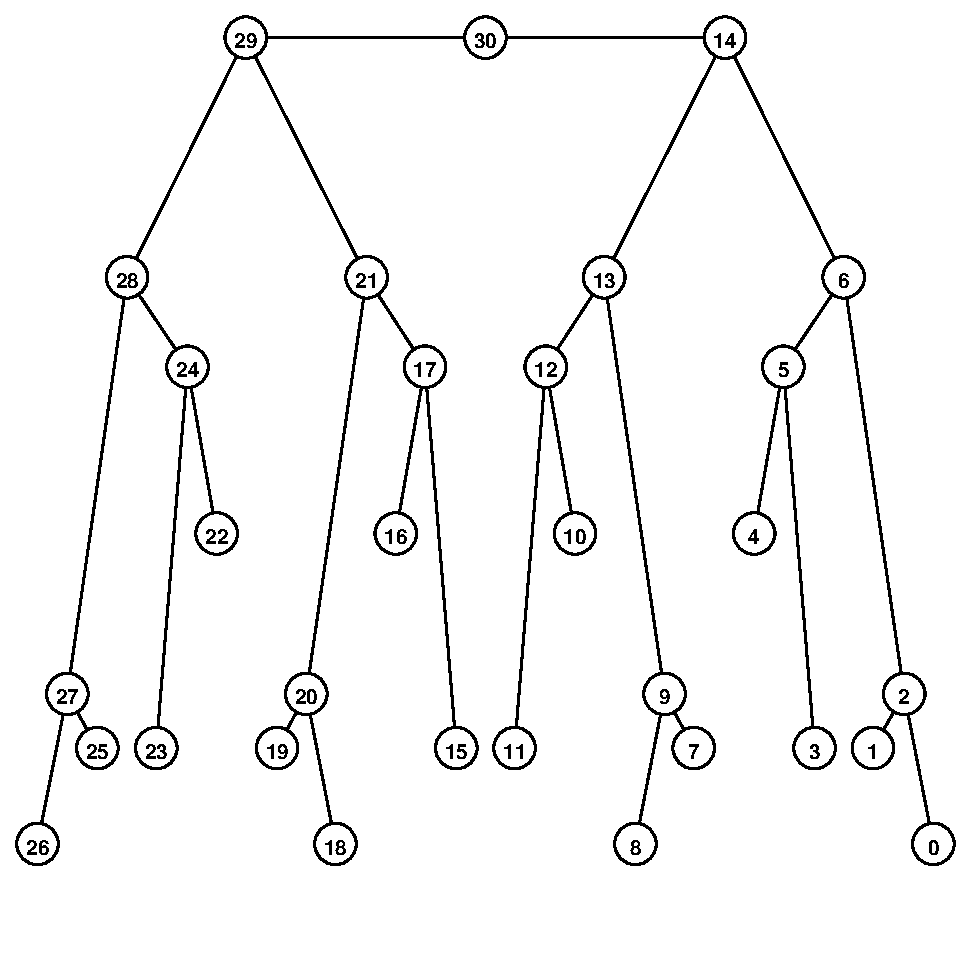
\psfig{file=../../ETree/doc/FS1.eps,height=3.00in,width=3.00in}
}
\fbox{
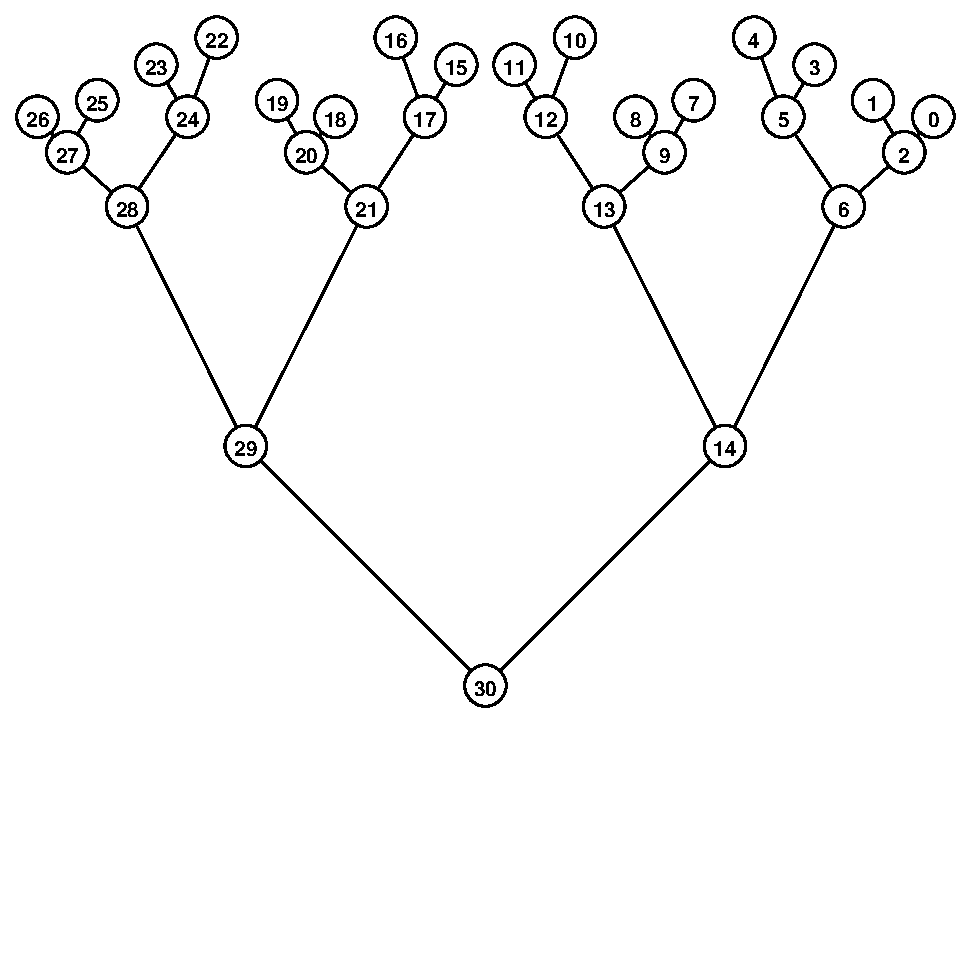
\psfig{file=../../ETree/doc/FS2.eps,height=3.00in,width=3.00in}
}
\end{center}
\end{figure}
%-----------------------------------------------------------------------
\item
\begin{verbatim}
testHeight msglvl msgFile inETreeFile 
\end{verbatim}
This driver program computes the height of the front tree with
respect to factor storage.
This quantity is the minimum amount of working storage 
for a forward sparse factorization.
\par
\begin{itemize}
\item
The {\tt msglvl} parameter determines the amount of output ---
taking {\tt msglvl >= 3} means the {\tt ETree} object is written
to the message file.
\item
The {\tt msgFile} parameter determines the message file --- if {\tt
msgFile} is {\tt stdout}, then the message file is {\it stdout},
otherwise a file is opened with {\it append} status to receive any
output data.
\item
The {\tt inETreeFile} parameter is the input file for the {\tt ETree}
object. It must be of the form {\tt *.etreef} or {\tt *.etreeb}.
The {\tt ETree} object is read from the file via the
{\tt ETree\_readFromFile()} method.
\end{itemize}
%-----------------------------------------------------------------------
\item
\begin{verbatim}
testIO msglvl msgFile inFile outFile
\end{verbatim}
This driver program reads and writes {\tt ETree} files, useful for
converting formatted files to binary files and vice versa.
One can also read in a {\tt ETree} file and print out just the 
header information (see the {\tt ETree\_writeStats()} method).
\par
\begin{itemize}
\item
The {\tt msglvl} parameter determines the amount of output ---
taking {\tt msglvl >= 3} means the {\tt ETree} object is written
to the message file.
\item
The {\tt msgFile} parameter determines the message file --- if {\tt
msgFile} is {\tt stdout}, then the message file is {\it stdout},
otherwise a file is opened with {\it append} status to receive any
output data.
\item
The {\tt inFile} parameter is the input file for the {\tt ETree}
object. It must be of the form {\tt *.etreef} or {\tt *.etreeb}.
The {\tt ETree} object is read from the file via the
{\tt ETree\_readFromFile()} method.
\item
The {\tt outFile} parameter is the output file for the {\tt ETree}
object. 
If {\tt outFile} is {\tt none} then the {\tt ETree} object is not
written to a file. 
Otherwise, the {\tt ETree\_writeToFile()} method is called to write
the object to 
a formatted file (if {\tt outFile} is of the form {\tt *.etreef}),
or
a binary file (if {\tt outFile} is of the form {\tt *.etreeb}).
\end{itemize}
%-----------------------------------------------------------------------
\item
\begin{verbatim}
testMaps msglvl msgFile inETreeFile outIVfile nthread type cutoff
\end{verbatim}
This program is used to construct an owners {\tt IV} that maps a
front to its owning thread or process.
The owners map {\tt IV} object is optionally written to a file.
\par
\begin{itemize}
\item
The {\tt msglvl} parameter determines the amount of output ---
taking {\tt msglvl >= 3} means the {\tt ETree} object is written
to the message file.
\item
The {\tt msgFile} parameter determines the message file --- if {\tt
msgFile} is {\tt stdout}, then the message file is {\it stdout},
otherwise a file is opened with {\it append} status to receive any
output data.
\item
The {\tt inETreeFile} parameter is the input file for the {\tt ETree}
object. It must be of the form {\tt *.etreef} or {\tt *.etreeb}.
The {\tt ETree} object is read from the file via the
{\tt ETree\_readFromFile()} method.
\item
The {\tt outIVFile} parameter is the output file for the 
owners map {\tt IV} object. 
If {\tt outIVFile} is {\tt none} then the {\tt IV} object is not
written to a file. 
Otherwise, the {\tt IV\_writeToFile()} method is called to write
the object to a formatted file (if {\tt outIVFile} 
is of the form {\tt *.ivf}), or a binary file 
(if {\tt outIVFile} is of the form {\tt *.ivb}).
\item
The {\tt nthread} parameter specifies the number of threads or
processes to be used.
\item
The {\tt type} parameter specifies the type of multisector.
\begin{itemize}
\item
{\tt type == 1} 
--- use {\tt ETree\_wrapMap()} to compute a wrap mapping.
\item
{\tt type == 2} 
--- use {\tt ETree\_balancedMap()} to compute a balanced mapping.
\item
{\tt type == 3} 
--- use {\tt ETree\_subtreeSubset()} 
    to compute a subtree-subset mapping.
\item
{\tt type == 4} 
--- use {\tt ETree\_ddMap()} to compute a domain decomposition map.
\end{itemize}
\item
{\tt cutoff} is a cutoff value for the multisector used only for
the domain decomposition map.
The cutoff defines the multisector, $0 \le \mbox{\tt cutoff} \le 1$.
If front {\tt J} has a subtree metric based on forward operations
that is greater than or equalt to {\tt cutoff} times the total
number of operations, then front {\tt J} belongs to the
multisector.
\end{itemize}
%-----------------------------------------------------------------------
\item
\begin{verbatim}
testMS msglvl msgFile inETreeFile outIVfile flag cutoff
\end{verbatim}
This program is used to extract a multisector from a front tree
{\tt ETree} object.
It partitions the vertices into domains and a multisector, where
each domain is a subtree of the elimination tree and the
multisector is the rest of the vertices.
The choice of the subtrees depends on the {\tt flag} and {\tt
cutoff} parameters --- it can be based on depth of a subtree or the
number of vertices, factor entries or factor operations associated
with the subtree.
The component ids {\tt IV} object is optionally written to a file.
Here is some sample output for {\tt BCSSTK30} ordered by nested
dissection, where the multisector is defined by subtree vertex
weight ({\tt flag = 2}) with {\tt cutoff = 0.125}.
\begin{verbatim}
 region  vertices    entries   operations   metric/(avg domain)
     0       1671     597058    255691396  0.797  2.201  3.967
     1       3104     255341     33205237  1.481  0.941  0.515
     2       3222     457255    116441261  1.537  1.685  1.806
     3       1514     194916     41940202  0.722  0.718  0.651
     4       2057     333186    100212056  0.981  1.228  1.555
     5         77       5040       356454  0.037  0.019  0.006
     6       1750     266166     62607526  0.835  0.981  0.971
     7       1887     325977    101994905  0.900  1.202  1.582
     8       3405     492662    125496320  1.624  1.816  1.947
     9       3413     501150    141423868  1.628  1.847  2.194
    10       3242     320220     51679456  1.546  1.180  0.802
    11       2118     238011     44427959  1.010  0.877  0.689
    12       1454     136777     18166107  0.694  0.504  0.282
    13         10        106         1168  0.005  0.000  0.000
 
                    nvtx   %         nzf   %           ops    %
 domains           27253 94.22   3526807 85.52    837952519 76.620
 schur complement   1671  5.78    597058 14.48    255691396 23.380
 total             28924         4123865         1093643915      
\end{verbatim}
Region {\tt 0} is the Schur complement, and there are thirteen
domains, eleven of good size.
A perfectly balanced tree would have eight domains using {\tt cutoff}
equal to 1/8.
It is interesting to see that the Schur complment contains only six
per cent of the vertices but almost one quarter the number of
operations.
\par
\begin{itemize}
\item
The {\tt msglvl} parameter determines the amount of output ---
taking {\tt msglvl >= 3} means the {\tt ETree} object is written
to the message file.
\item
The {\tt msgFile} parameter determines the message file --- if {\tt
msgFile} is {\tt stdout}, then the message file is {\it stdout},
otherwise a file is opened with {\it append} status to receive any
output data.
\item
The {\tt inETreeFile} parameter is the input file for the {\tt ETree}
object. It must be of the form {\tt *.etreef} or {\tt *.etreeb}.
The {\tt ETree} object is read from the file via the
{\tt ETree\_readFromFile()} method.
\item
The {\tt outIVFile} parameter is the output file for the {\tt IV}
object. 
If {\tt outIVFile} is {\tt none} then the {\tt IV} object is not
written to a file. 
Otherwise, the {\tt IV\_writeToFile()} method is called to write
the object to a formatted file (if {\tt outIVFile} 
is of the form {\tt *.ivf}), or a binary file 
(if {\tt outIVFile} is of the form {\tt *.ivb}).
\item
The {\tt flag} parameter specifies the type of multisector.
\begin{itemize}
\item
{\tt flag == 1} --- the multisector is based on the depth of the
front, i.e., if the front is more than {\tt depth} steps removed
from the root, it forms the root of a domain.
\item
{\tt flag == 2} --- the multisector is based on the number of
vertices in a subtree, i.e., if the subtree rooted at a front
contains more than {\tt cutoff} times the total number of vertices,
it is a domain.
\item
{\tt flag == 3} --- the multisector is based on the number of
factor entries in a subtree, i.e., if the subtree rooted at a front
contains more than {\tt cutoff} times the total number of factor
entries, it is a domain.
\item
{\tt flag == 4} --- the multisector is based on the number of
factor operations in a subtree, i.e., if the subtree rooted at a front
contains more than {\tt cutoff} times the total number of factor
operations, it is a domain.
\end{itemize}
\item
{\tt cutoff} is a cutoff value for the multisector, see above
description when {\tt flag} equals {\tt 1}, {\tt 2} or {\tt 3}.
\end{itemize}
%-----------------------------------------------------------------------
\item
\begin{verbatim}
testStats msglvl msgFile inETreeFile labelflag radius firstEPSfile secondEPSfile
\end{verbatim}
This driver program computes one of five metrics associated with a
front tree and writes an EPS file that illustrates the metric overlaid
on the tree structure.
It first reads in a front tree object and 
a graph file.
There are six possible plots:
\begin{center}
\begin{tabular}{c|l}
{\tt metricType} & type of metric \\ \hline
0 & no metric, just a tree plot \\
1 & \# of nodes in a front \\
2 & \# of original matrix entries in a front \\
3 & \# of factor matrix entries in a front \\
4 & \# of forward factor operations in a front \\
5 & \# of backward factor operations in a front 
\end{tabular}
\end{center}
The maximum value of the metric creates a circle with radius
{\tt rmax}, and all other nodes have circles with their area
relative to this largest circle.
See Figure~\ref{fig-GRD7x7x7-metrics} contains four plots,
each used {\tt heightflag = 'D'}, {\tt coordflag = 'P'},
{\tt rmax = 20} and {\tt labelflag = 0}.
\par
\begin{itemize}
\item
The {\tt msglvl} parameter determines the amount of output ---
taking {\tt msglvl >= 3} means the {\tt ETree} object is written
to the message file.
\item
The {\tt msgFile} parameter determines the message file --- if {\tt
msgFile} is {\tt stdout}, then the message file is {\it stdout},
otherwise a file is opened with {\it append} status to receive any
output data.
\item
The {\tt inETreeFile} parameter is the input file for the {\tt ETree}
object. It must be of the form {\tt *.etreef} or {\tt *.etreeb}.
The {\tt ETree} object is read from the file via the
{\tt ETree\_readFromFile()} method.
\item
The {\tt inGraphFile} parameter is the input file for the {\tt Graph}
object. It must be of the form {\tt *.graphf} or {\tt *.graphb}.
The {\tt Graph} object is read from the file via the
{\tt Graph\_readFromFile()} method.
\item
The {\tt outEPSfile} parameter is the name of the EPS file 
to hold the tree.
\item
The {\tt metricType} parameter defines the type of metric to be
illustrated. See above for values.
\item
For information about the {\tt heightflag} and {\tt coordflag}
parameters, see Section~\ref{subsection:Tree:proto:drawing}.
\item
If {\tt labelflag = 1}, the node ids are written on the nodes
in the two plots.
\item
The {\tt fontscale} parameter is the font size when labels are
drawn.
\end{itemize}
\begin{figure}[htbp]
\caption{{\sc GRD7x7x7}: Four tree plots for a $7 \times 7 \times 7$
grid matrix ordered using nested dissection.
The top left tree measure number of original matrix entries in a front.
The top right tree measure number of factor matrix entries in a front.
The bottom left tree measure number of factor operations in a front
for a forward looking factorization, e.g., forward sparse.
The bottom right tree measure number of factor operations in a front
for a backward looking factorization, e.g., general sparse.}
\label{fig-GRD7x7x7-metrics}
\begin{center}
\fbox{
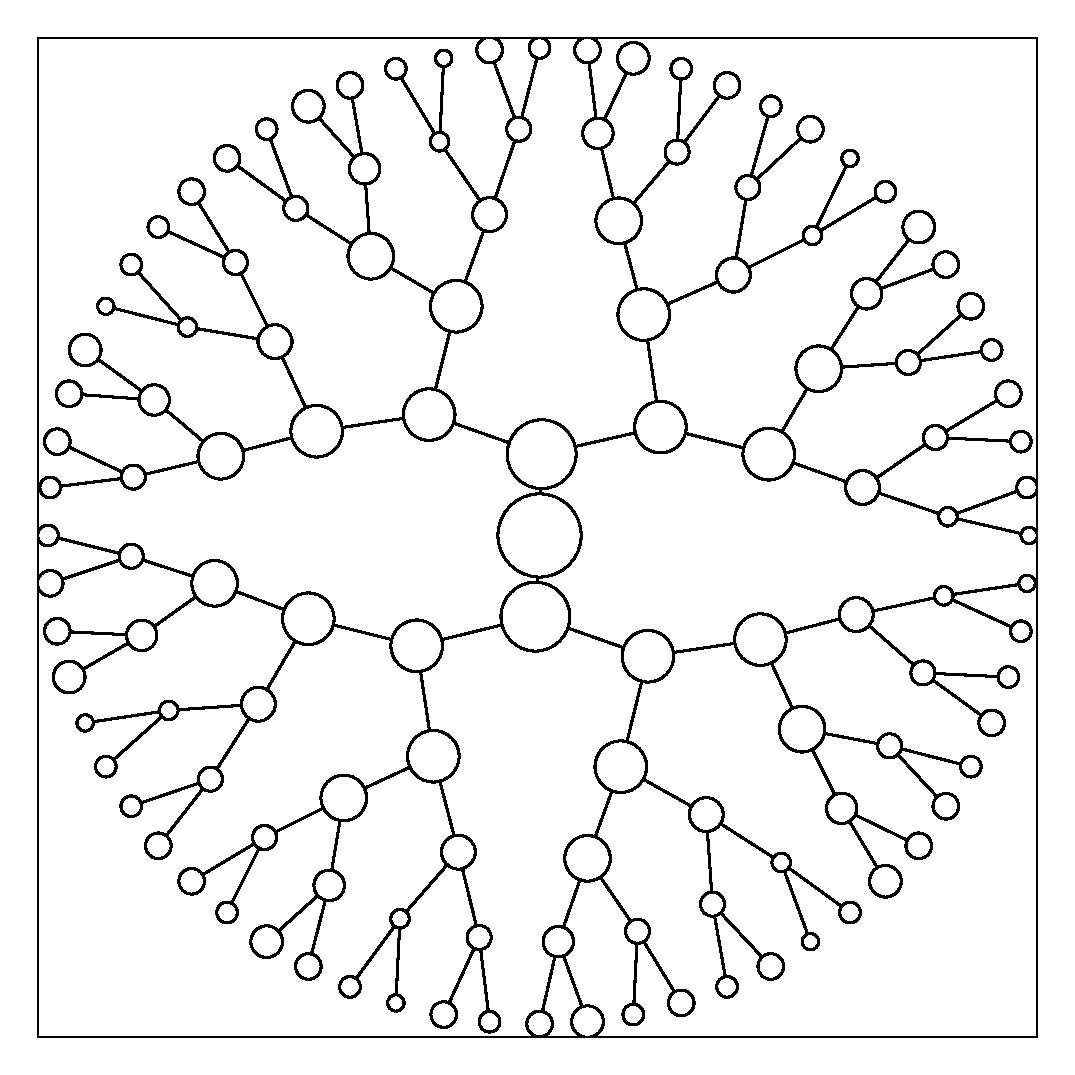
\psfig{file=../../ETree/doc/GRD7x7x7_nzA.eps,height=3.00in,width=3.00in}
}
\fbox{
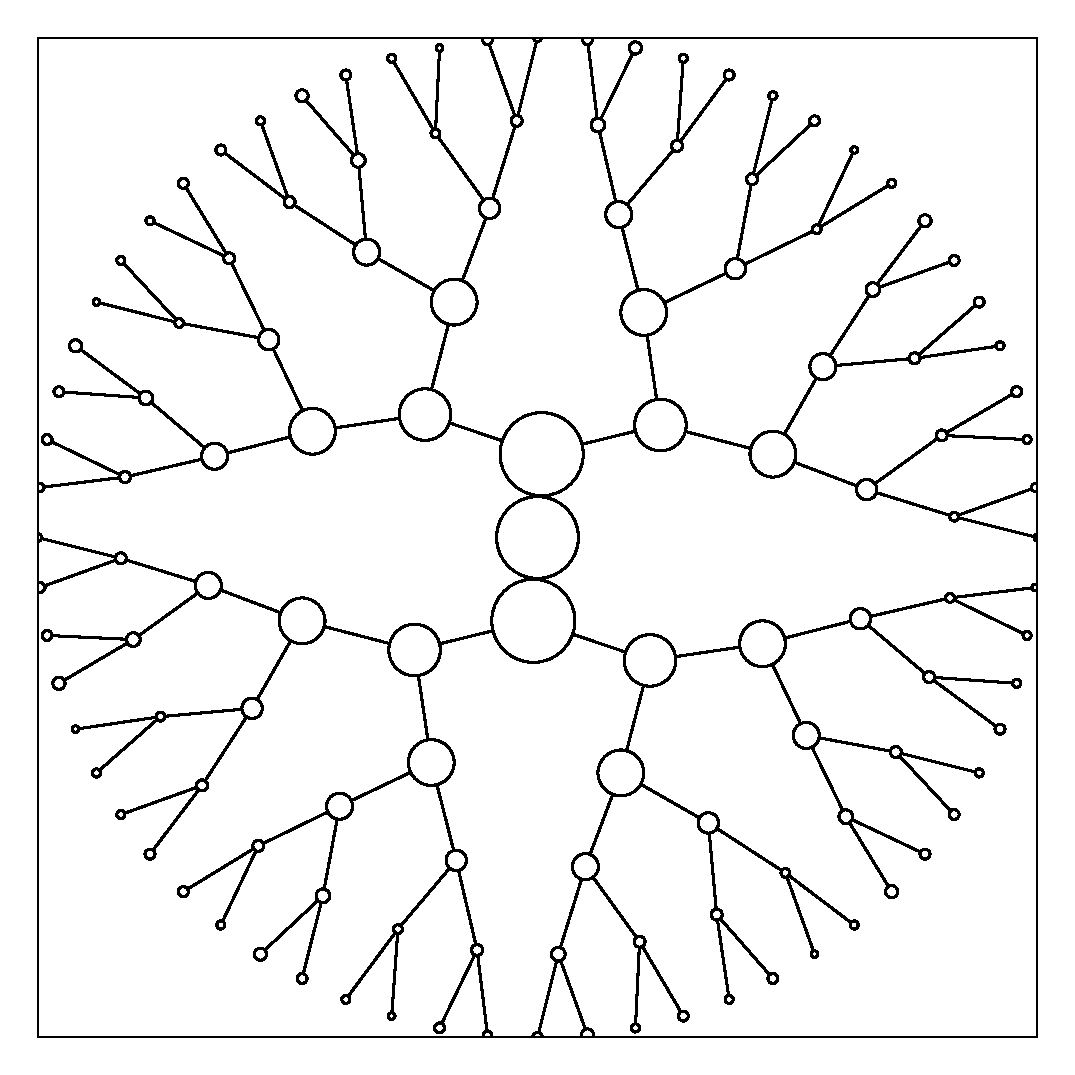
\psfig{file=../../ETree/doc/GRD7x7x7_nzF.eps,height=3.00in,width=3.00in}
}
\par
\fbox{
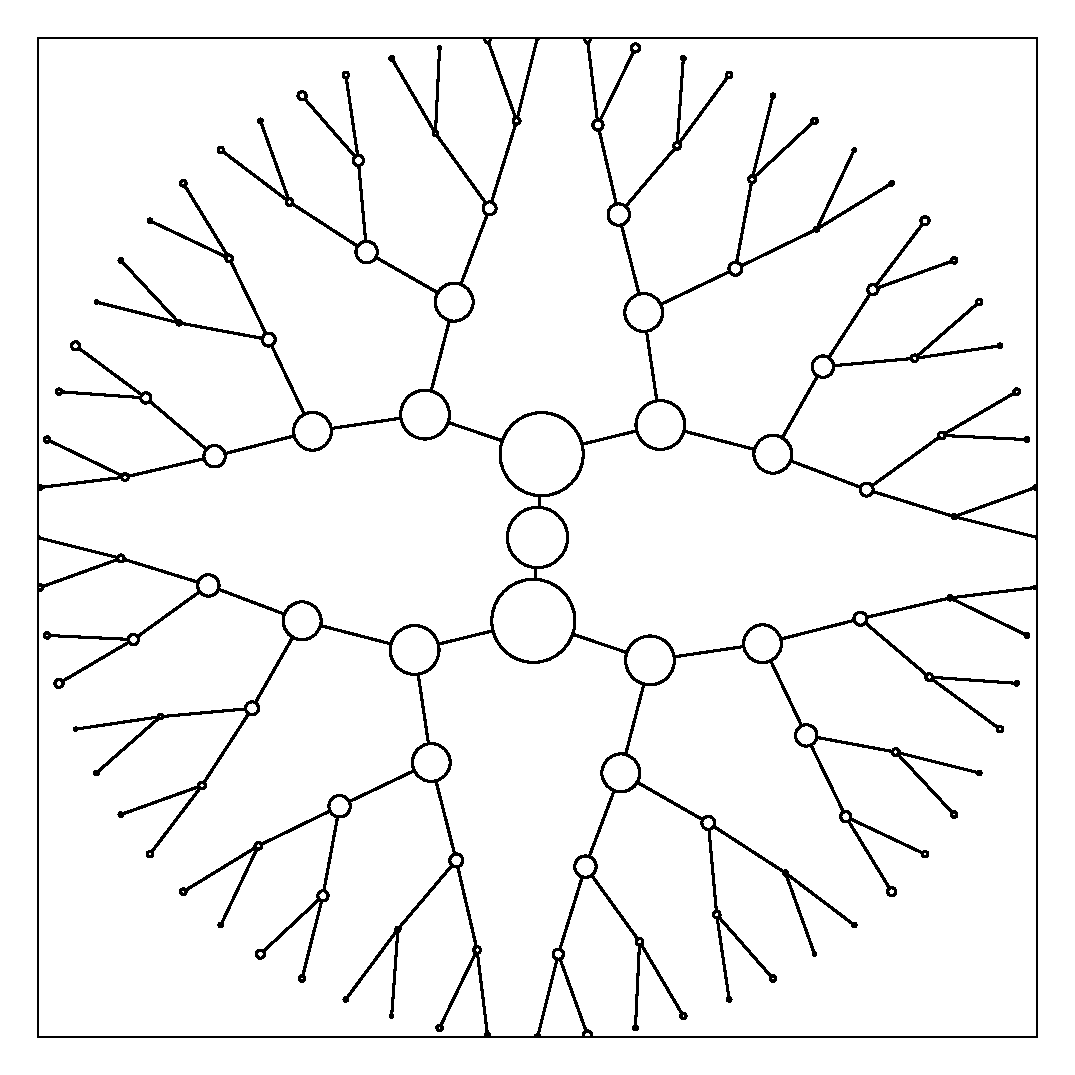
\psfig{file=../../ETree/doc/GRD7x7x7_forwops.eps,height=3.00in,width=3.00in}
}
\fbox{
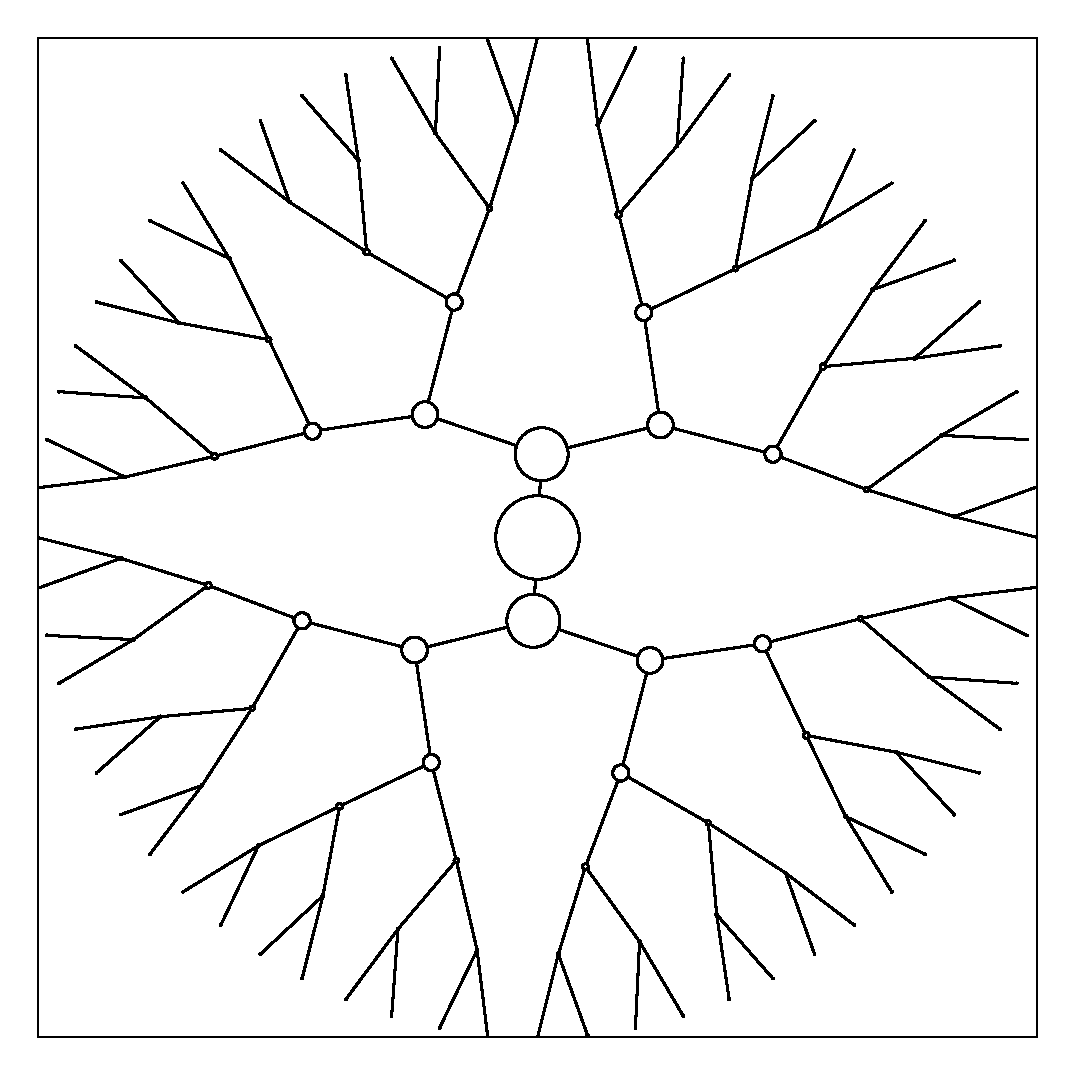
\psfig{file=../../ETree/doc/GRD7x7x7_backops.eps,height=3.00in,width=3.00in}
}
\end{center}
\end{figure}
%-----------------------------------------------------------------------
\item
\begin{verbatim}
testStorage msglvl msgFile inETreeFile inGraphFile 
\end{verbatim}
This driver program is used to evaluate the working storage for the
left-looking general sparse and multifrontal algorithms using the
natural post-order traversal of the front tree.
The output is in matlab format to produce a plot.
An example is found below.
\begin{center}
\makebox{
% \psfig{file=workingStorage.eps,width=3.0in,height=2.40in}
\psfig{file=../../ETree/doc/workingStorage.eps,width=3.0in,height=2.40in}
}
\end{center}
\par
\begin{itemize}
\item
The {\tt msglvl} parameter determines the amount of output ---
taking {\tt msglvl >= 3} means the {\tt ETree} object is written
to the message file.
\item
The {\tt msgFile} parameter determines the message file --- if {\tt
msgFile} is {\tt stdout}, then the message file is {\it stdout},
otherwise a file is opened with {\it append} status to receive any
output data.
\item
The {\tt inETreeFile} parameter is the input file for the {\tt ETree}
object. It must be of the form {\tt *.etreef} or {\tt *.etreeb}.
The {\tt ETree} object is read from the file via the
{\tt ETree\_readFromFile()} method.
\item
The {\tt inGraphFile} parameter is the input file for the {\tt Graph}
object. It must be of the form {\tt *.graphf} or {\tt *.graphb}.
The {\tt Graph} object is read from the file via the
{\tt Graph\_readFromFile()} method.
\end{itemize}
%-----------------------------------------------------------------------
\item
\begin{verbatim}
testTransform msglvl msgFile inETreeFile inGraphFile 
              outETreeFile maxzeros maxsize seed
\end{verbatim}
This driver program is used to transform a front tree {\tt ETree}
object into a (possibly) merged and (possibly) split front tree.
{\it Merging} the front tree means combining fronts together
that do not introduce more than {\tt maxzeros} zero entries in a
front. (See \cite{ash89-relaxed} and \cite{duf83-multifrontal}
for a description of this supernode amalgamation or relaxation.)
{\it Splitting} a front means breaking a front up into a chain of
smaller fronts; this allows more processors to work on the original
front in a straightforward manner.
The new front tree is optionally written to a file.
Here is some output for the {\tt R3D13824} matrix using
{\tt maxzeros = 1000} and {\tt maxsize = 64}.
\begin{verbatim}
                  CPU  #fronts  #indices  #entries       #ops
 original  :              6001    326858   3459359   1981403337 
 merge one :    0.209     3477    158834   3497139   2000297117 
 merge all :    0.136      748     95306   3690546   2021347776 
 merge any :    0.073      597     85366   3753241   2035158539 
 split     :    0.202      643    115139   3753241   2035158539 
 final     :    3.216      643    115128   3752694   2034396840 
\end{verbatim}
Note how the number of fronts, front indices, factor entries and
factor operations change after each step.
Merging chains (the {\tt merge one} line) halves 
the number of fronts while increasing operations by 1\%.
Merging all children when possible 
(the {\tt merge all} line)
reduces the number of fronts by a factor of 5 
while increasing operations by another 1\%.
Merging any other children (the {\tt merge any} line)
has another additional effect.
Splitting the fronts increases the number of fronts slightly, 
but appears not to change the factor entries or operation counts. 
This is false, as the final step computes the symbolic
factorization for the last front tree and updates the boundary
sizes of the fronts. 
We see that the number of indices, entries and factor operations 
actually decrease slightly due to the split fronts.
\par
\begin{itemize}
\item
The {\tt msglvl} parameter determines the amount of output ---
taking {\tt msglvl >= 3} means the {\tt ETree} object is written
to the message file.
\item
The {\tt msgFile} parameter determines the message file --- if {\tt
msgFile} is {\tt stdout}, then the message file is {\it stdout},
otherwise a file is opened with {\it append} status to receive any
output data.
\item
The {\tt inETreeFile} parameter is the input file for the {\tt ETree}
object. It must be of the form {\tt *.etreef} or {\tt *.etreeb}.
The {\tt ETree} object is read from the file via the
{\tt ETree\_readFromFile()} method.
\item
The {\tt inGraphFile} parameter is the input file for the {\tt Graph}
object. It must be of the form {\tt *.graphf} or {\tt *.graphb}.
The {\tt Graph} object is read from the file via the
{\tt Graph\_readFromFile()} method.
\item
The {\tt outETreeFile} parameter is the output file for the {\tt ETree}
object. 
If {\tt outETreeFile} is {\tt none} then the {\tt ETree} object is not
written to a file. 
Otherwise, the {\tt ETree\_writeToFile()} method is called to write
the object to a formatted file (if {\tt outETreeFile} 
is of the form {\tt *.etreef}), or a binary file 
(if {\tt outETreeFile} is of the form {\tt *.etreeb}).
\item
The {\tt maxzeros} parameter is an upper bound on the number of
logically zero entries that will be allowed in a new front.
\item
The {\tt maxsize} parameter is an upper bound on the number of
vertices in a front --- any original front that contains more than
{\tt maxsize} vertices will be broken up into smaller fronts.
\item
{\tt seed} is a seed for a random number generator.
\end{itemize}
%-----------------------------------------------------------------------
\end{enumerate}
